\chapter{Grid Description}
\label{chap:mpas_grid_description}

This chapter provides a brief introduction to the common types of grids used in the MPAS framework. 

The MPAS grid system requires the definition of seven elements. These seven elements are composed of two types of {\it cells}, two types of {\it lines}, and three types of {\it points}. These elements are depicted in Figure \ref{figure:variablePosition} and defined in Table \ref{table:variablePosition}.  These elements can be defined on either the plane or the surface of the sphere. The two types of cells form two meshes, a primal mesh composed of Voronoi regions and a dual mesh composed of Delaunay triangles. Each corner of a primal mesh cell is uniquely associated with the ``center'' of a dual mesh cell and vice versa. So we define the two mesh as either a primal mesh (composed of cells $P_i$) or a dual mesh (composed of cells $D_v$). The center of any primal mesh cell, $P_i$, is denoted by ${\bf x}_i$ and the center of any the dual mesh cell, $D_v$, is denoted by ${\bf x}_v$. The boundary of a given primal mesh cell $P_i$ is composed of the set of lines that connect the ${\bf x}_v$ locations of associated dual mesh cells $D_v$. Similarly, the boundary of a given dual mesh cell $D_v$ is composed of the set of lines that connect the ${\bf x}_i$ locations of the associated primal mesh cells $P_i$. 

As shown in Figure \ref{figure:variablePosition}, a line segment that connects two primal mesh cell centers is uniquely associated with a line segment that connects two dual mesh cell centers. We assume that these two line segments cross and the point of intersection is labeled as ${\bf x}_e$. In addition, we assume that these two line segments are orthogonal as indicated in Figure \ref{figure:variablePosition}. Each ${\bf x}_e$ is associated with two distances: $d_e$ measures the distance between the primal mesh cells sharing ${\bf x}_e$ and $l_e$ measures the distance between the dual mesh cells sharing ${\bf x}_e$.

Since the two line segments crossing at ${\bf x}_e$ are orthogonal, these line segments form a convenient local coordinate system for each edge. At each ${\bf x}_e$ location a unit vector ${\bf n}_e$ is defined to be parallel to the line connecting primal mesh cells. A second unit vector ${\bf t}_e$ is defined such that ${\bf t}_e = {\bf k} \times {\bf n}_e$.

In addition to these seven element types, we require the definition of {\it sets of elements}. In all, eight different types of sets are required and these are defined and explained in Table \ref{table:gridConnectivity} and Figure \ref{figure:gridConnectivity}. The notation is always of the form of, for example, $i \in CE(e)$, where the LHS indicates the type of element to be gathered (cells) based on the RHS relation to another type of element (edges).

Table \ref{table:gridFileName} provides the names of all {\it elements} and all {\it sets of elements} as used in the MPAS framework.  Elements appear twice in the table when described in the grid file in more than one way, e.g. points are described with both cartesian and latitude/longitude coordinates. An ``ncdump -h'' of any MPAS grid, output or restart file will contain all variable names shown in second column of Table  \ref{table:gridFileName}.


\begin{table}[t]
\caption{Definition of elements used to build the MPAS grid.}
\label{table:variablePosition}
\begin{center}
\begin{tabular}{lll}
\hline\hline
$Element$ & $Type$ & $Definition$\\
\hline
 ${\bf x}_i$   & point             & location of center of primal-mesh cells \\
 ${\bf x}_v$  &  point            & location of center of dual-mesh cells \\
 ${\bf x}_e$  & point             & location of edge points where velocity is defined \\
 $d_{e}$       & line segment & distance between neighboring ${\bf x}_i$ locations \\
 $l_{e}$       & line segment & distance between neighboring ${\bf x}_v$ locations \\
 $P_i$         & cell                 & a cell on the primal-mesh \\
 $D_v$        & cell                 & a cell on the dual-mesh \\
\hline
\end{tabular}
\end{center}
\end{table}
%
\begin{table}[t]
\caption{Definition of element groups used to reference connections in the MPAS grid. Examples are provided in Figure \ref{figure:gridConnectivity}.}
\label{table:gridConnectivity}
\begin{center}
\begin{tabular}{lll}
\hline\hline
$Syntax$ & $ouptut$\\
\hline
 $e \in EC(i) $   & set of edges that define the boundary of $P_i$. \\
 $e \in EV(v) $     & set of edges that define the boundary of $D_v$. \\
 $i \in CE(e) $                 & two primal-mesh cells that share edge $e$. \\
 $i \in CV(v) $  &  set of primal-mesh cells that form the vertices of dual mesh cell $D_v$. \\
 $v\in VE(e) $  & the two dual-mesh cells that share edge $e$. \\
 $v \in VI(i) $   & the set of dual-mesh cells that form the vertices of primal-mesh cell $P_i$. \\
 $e \in ECP(e)$ & edges of cell pair meeting at edge $e$. \\
 $e \in EVC(v,i)$ & edge pair associated with vertex $v$ and mesh cell $i$. \\
\hline
\end{tabular}
\end{center}
\end{table}
%

\begin{table}[t]
\caption{Variable names used to describe a MPAS grid.}
\label{table:gridFileName}
\begin{center}
\begin{tabular}{llll}
\hline\hline
$Element$ & $Name$ & $Size$ & $Comment$\\
\hline
 ${\bf x}_i$   & \{x,y,z\}Cell          & nCells  & cartesian location of ${\bf x}_i$  \\
 ${\bf x}_i$   & \{lon,lat\}Cell        & nCells  & longitude and latitude of  ${\bf x}_i$  \\
 ${\bf x}_v$   & \{x,y,z\}Vertex      & nVertices  & cartesian location of ${\bf x}_v$  \\
 ${\bf x}_v$   & \{lon,lat\}Vertex    & nVertices  & longitude and latitude of  ${\bf x}_v$  \\
 ${\bf x}_e$   & \{x,y,z\}Edge          & nEdges  & cartesian location of ${\bf x}_e$  \\
 ${\bf x}_e$   & \{lon,lat\}Edge        & nEdges  & longitude and latitude of  ${\bf x}_e$  \\
 $d_{e}$       & dcEdge                   & nEdges  & distance between ${\bf x}_i$ locations\\
 $l_{e}$         & dvEdge             & nEdges &  distance between ${\bf x}_v$ locations \\
  &  & & \\
 $e \in EC(i) $   &  edgesOnCell  & (nEdgesMax,nCells) & edges that define $P_i$. \\
 $e \in EV(v) $     & edgesOnVertex &  (3,nCells) & edges that define $D_v$. \\
 $i \in CE(e) $      & cellsOnEdge &  (2,nEdges) &  primal-mesh cells that share edge $e$. \\
 $i \in CV(v) $  &   cellsOnVertex &  (3,nVertices) &  primal-mesh cells that define $D_v$. \\
 $v\in VE(e) $  & verticesOnEdge &  (2,nEdges) &    dual-mesh cells that share edge $e$. \\
 $v \in VI(i) $   & verticesOnCell &  (nEdgesMax,nCells) & vertices that define $P_i$. \\
\hline
\end{tabular}
\end{center}
\end{table}
%


%
\begin{figure}[t]
  \noindent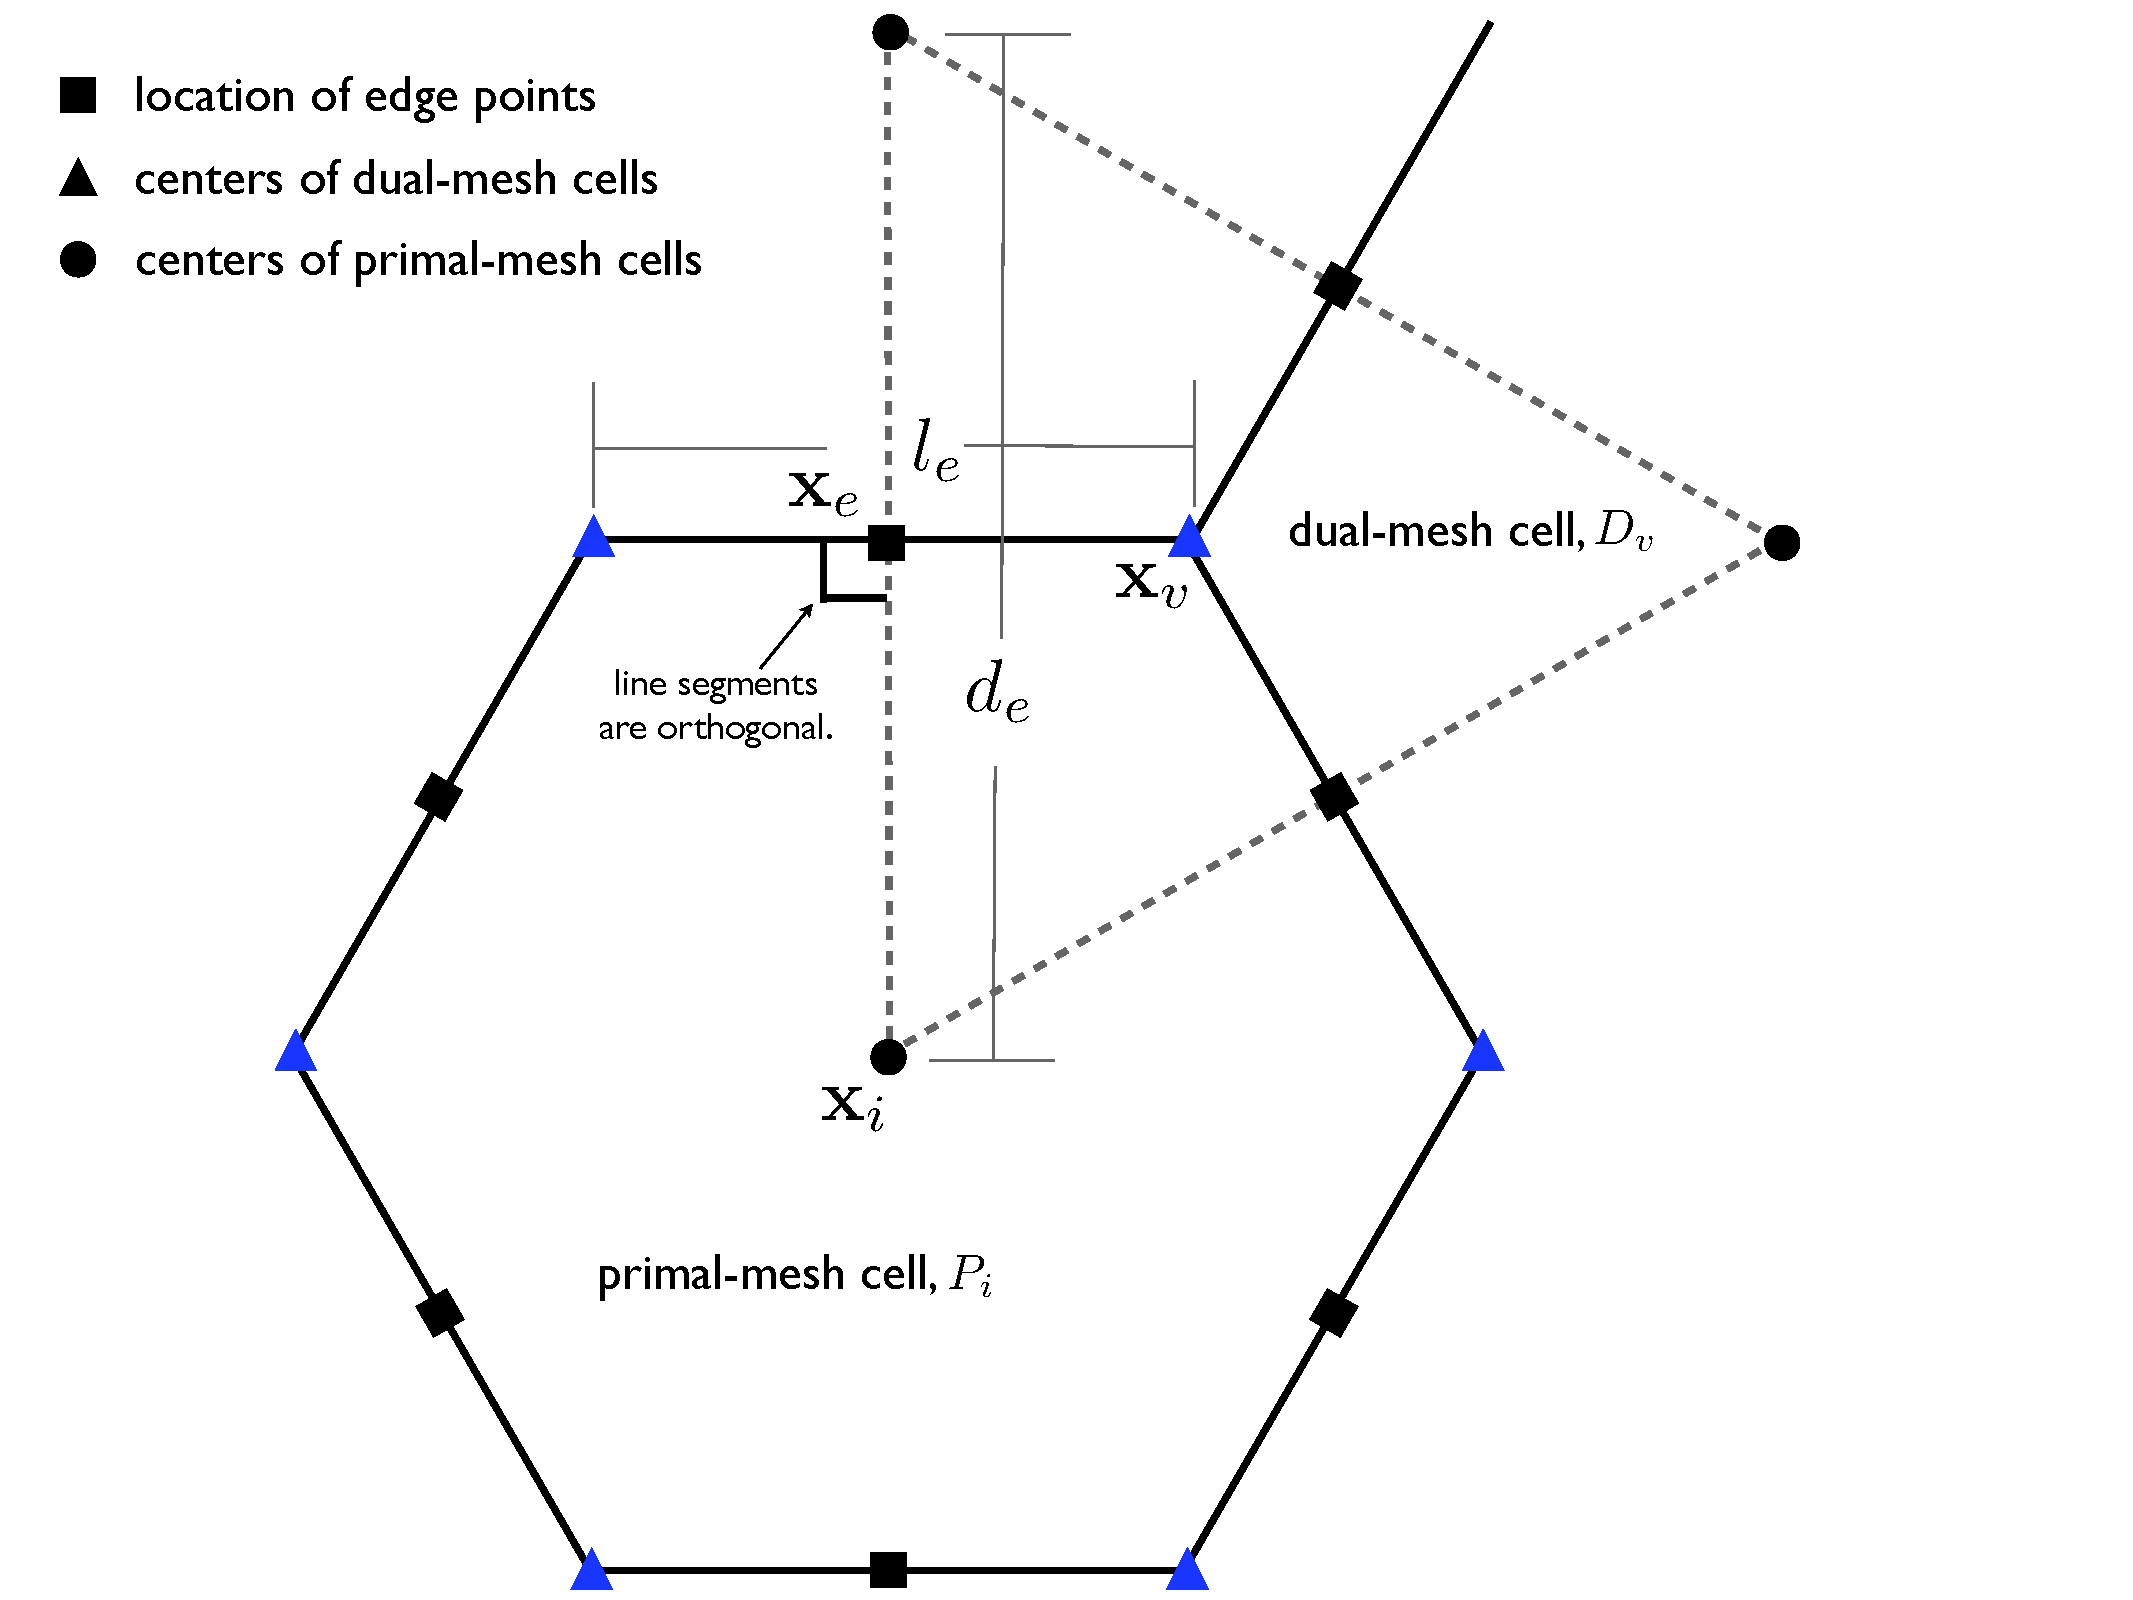
\includegraphics[width=16cm,angle=0]{./shared/figures/variablePosition.pdf}\\
  \caption{Definition of elements used to build the MPAS grid. Also see Table \ref{table:variablePosition}.}
  \label{figure:variablePosition}
\end{figure}

%
\begin{figure}[t]
   \noindent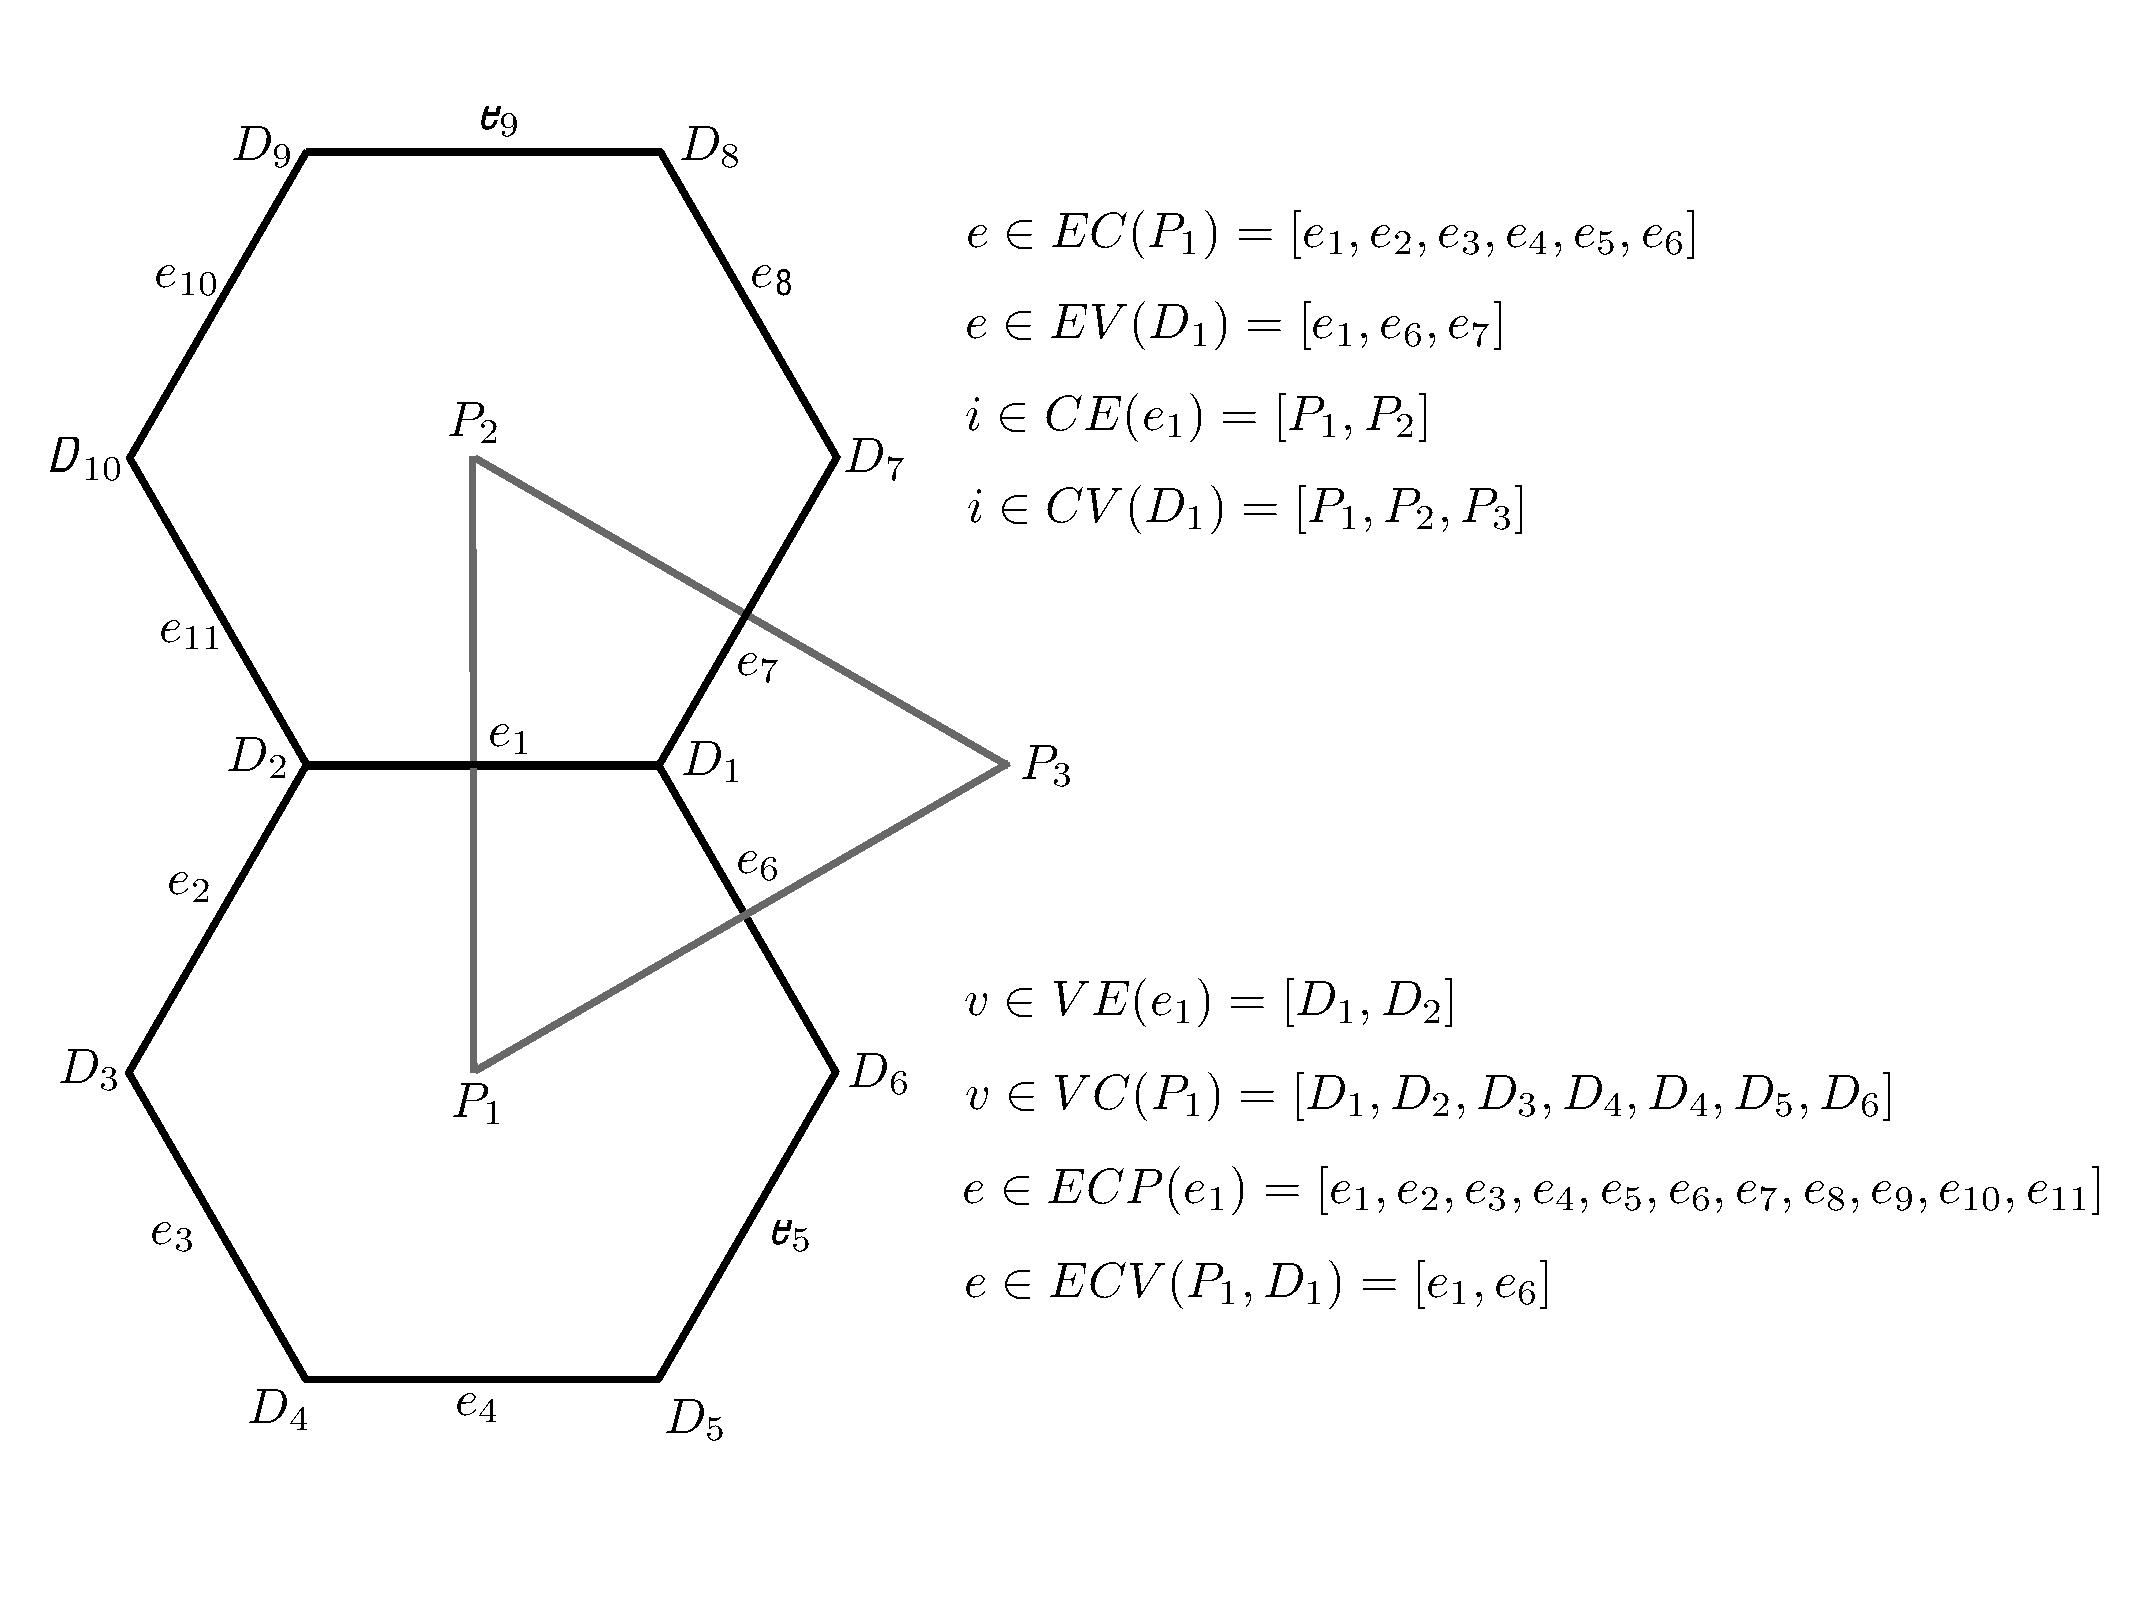
\includegraphics[width=16cm,angle=0]{./shared/figures/gridConnectivity.pdf}\\
  \caption{Definition of element groups used to reference connections in the MPAS grid. Also see Table \ref{table:gridConnectivity}.}
  \label{figure:gridConnectivity}
\end{figure}


